\documentclass{beamer}

% Should be documentclass beamer

\mode<presentation>
{
%  \usetheme[hideothersubsections]{PaloAlto}
  \usetheme{metropolis}
  \setbeamercovered{transparent}
}

\usepackage{amsfonts}
\usepackage{amsmath}
\usepackage{amssymb}
\usepackage{color}
\usepackage{tikz}
\usepackage{pgfplots}
\usepackage{listings}
\usepackage{courier}
%\usepackage[utf8]{inputenc}
%\usepackage[russian]{babel}

\lstset{
  numbers=left,
  basicstyle=\ttfamily\footnotesize,
  numberstyle=\tiny\color{gray},
  stepnumber=1,
  numbersep=10pt,
}

\newcommand{\iu}{\ensuremath{\mathrm{i}}}
\newcommand{\bbR}{\mathbb{R}}
\newcommand{\bbC}{\mathbb{C}}
\newcommand{\calV}{\mathcal{V}}
\newcommand{\calW}{\mathcal{W}}
\newcommand{\macheps}{\epsilon_{\mathrm{mach}}}
\newcommand{\matlab}{\textsc{Matlab}}

\newcommand{\ddiag}{\operatorname{diag}}
\newcommand{\fl}{\operatorname{fl}}
\newcommand{\nnz}{\operatorname{nnz}}
\newcommand{\tr}{\operatorname{tr}}
\renewcommand{\vec}{\operatorname{vec}}

\newcommand{\vertiii}[1]{{\left\vert\kern-0.25ex\left\vert\kern-0.25ex\left\vert #1
    \right\vert\kern-0.25ex\right\vert\kern-0.25ex\right\vert}}
\newcommand{\ip}[2]{\langle #1, #2 \rangle}
\newcommand{\ipx}[2]{\left\langle #1, #2 \right\rangle}
\newcommand{\order}[1]{O( #1 )}

\newcommand{\kron}{\otimes}


\newcommand{\hdr}[2]{
  \title[CS 5220, Fall 2017]{CS 5220: #2}
  \author{David Bindel}
  \date{#1}
}


\hdr{2017-10-24}{Iterations and Sparse LA}

\begin{document}

\begin{frame}
  \titlepage
\end{frame}

% Resources:
% - Books -- Templates and company
% - Packages: PETSc and Trilinos (includes Hypre, ...); SLEPc for eigs
% - ACTS collection
% - Survey of parallel linear algebra software

\begin{frame}
  \frametitle{World of Linear Algebra}

  \begin{itemize}
  \item Dense methods (last week)
    \begin{itemize}
    \item Direct representation of matrices with
      simple data structures (no need for indexing data structure)
    \item Mostly $O(n^3)$ factorization algorithms
    \end{itemize}
  \item Sparse direct methods (Thurs)
    \begin{itemize}
    \item Direct representation, keep only the nonzeros
    \item Factorization costs depend on problem structure
      (1D cheap; 2D reasonable; 3D gets expensive; not easy to give a general
      rule, and NP hard to order for optimal sparsity)
    \item Robust, but hard to scale to large 3D problems
    \end{itemize}
  \item Iterative methods (today and Thurs)
    \begin{itemize}
    \item Only {\em need} $y = Ax$ (maybe $y = A^T x$)
    \item Produce successively better (?) approximations
    \item Good convergence depends on {\em preconditioning}
    \item Best preconditioners are often hard to parallelize
    \end{itemize}
  \end{itemize}

\end{frame}


\begin{frame}[fragile]
  \frametitle{Linear Algebra Software: MATLAB}
  
\begin{lstlisting}
% Dense (LAPACK)
[L,U] = lu(A);
x = U\(L\b);

% Sparse direct (UMFPACK + COLAMD)
[L,U,P,Q] = lu(A);
x = Q*(U\(L\(P*b)));

% Sparse iterative (PCG + incomplete Cholesky)
tol = 1e-6;
maxit = 500;
R = cholinc(A,'0');
x = pcg(A,b,tol,maxit,R',R);
\end{lstlisting}

\end{frame}


\begin{frame}
  \frametitle{Linear Algebra Software: the Wider World}

  \begin{itemize}
  \item Dense: LAPACK, ScaLAPACK, PLAPACK
  \item Sparse direct: UMFPACK, TAUCS, SuperLU, MUMPS, Pardiso, SPOOLES, ...
  \item Sparse iterative: too many!
  \item Sparse mega-libraries
    \begin{itemize}
    \item PETSc (Argonne, object-oriented C)
    \item Trilinos (Sandia, C++)
    \end{itemize}
  \item Good references:
    \begin{itemize}
    \item {\em Templates for the Solution of Linear Systems} 
      (on Netlib)
    \item Survey on ``Parallel Linear Algebra Software'' \\
      (Eijkhout, Langou, Dongarra -- look on Netlib)
    \item ACTS collection at NERSC
    \end{itemize}
  \end{itemize}
\end{frame}


\begin{frame}
  \frametitle{Software Strategies: Dense Case}

  Assuming you want to {\em use} (vs develop) dense LA code:
  \begin{itemize}
  \item Learn enough to identify right algorithm \\
    (e.g. is it symmetric? definite? banded? etc)
  \item Learn high-level organizational ideas
  \item Make sure you have a good BLAS
  \item Call LAPACK/ScaLAPACK!
  \item For $n$ large: wait a while
  \end{itemize}

\end{frame}


\begin{frame}
  \frametitle{Software Strategies: Sparse Direct Case}

  Assuming you want to use (vs develop) sparse LA code
  \begin{itemize}
  \item Identify right algorithm (mainly Cholesky vs LU)
  \item Get a good solver (often from list)
    \begin{itemize}
    \item You {\em don't} want to roll your own!
    \end{itemize}
  \item {\em Order your unknowns} for sparsity
    \begin{itemize}
    \item Again, good to use someone else's software!
    \end{itemize}
  \item For $n$ large, 3D: get lots of memory and wait
  \end{itemize}

\end{frame}


\begin{frame}
  \frametitle{Software Strategies: Sparse Iterative Case}

  Assuming you want to use (vs develop) sparse LA software...
  \begin{itemize}
  \item Identify a good algorithm (GMRES? CG?)
  \item Pick a good preconditioner
    \begin{itemize}
    \item Often helps to know the application
    \item ... {\em and} to know how the solvers work!
    \end{itemize}
  \item Play with parameters, preconditioner variants, etc...
  \item Swear until you get acceptable convergence?
  \item Repeat for the next variation on the problem
  \end{itemize}

  \vspace{5mm}
  Frameworks (e.g. PETSc or Trilinos) speed experimentation.

\end{frame}


\begin{frame}
  \frametitle{Software Strategies: Stacking Solvers}

  (Typical) example from a bone modeling package:
  \begin{itemize}
  \item Outer load stepping loop
  \item Newton method corrector for each load step
  \item Preconditioned CG for linear system
  \item Multigrid preconditioner
  \item Sparse direct solver for coarse-grid solve (UMFPACK)
  \item LAPACK/BLAS under that
  \end{itemize}

  \vspace{5mm}
  First three are high level --- I used a scripting language (Lua).

\end{frame}


\begin{frame}
  \frametitle{Iterative Idea}

  \begin{center}
    \begin{tikzpicture}[y=-1cm,scale=0.8]

% objects at depth 50:
\draw[->,black] (6.19125,4.36563) +(-143:1.19063) arc (-143:-37:1.19063);
\draw[->,black] (11.43,4.36563) +(-143:1.19063) arc (-143:-37:1.19063);
\filldraw[blue] (13.7795,4.1275) circle (0.0635cm);
\filldraw[blue] (8.89,3.33375) circle (0.0635cm);
\filldraw[blue] (3.81,2.54) circle (0.0635cm);
\filldraw[black] (3.14325,4.445) circle (0.0635cm);
\filldraw[black] (8.255,4.445) circle (0.0635cm);
\filldraw[black] (13.335,4.445) circle (0.0635cm);
\draw[arrows=to-to,black] (2.54,2.54) -- (2.54,5.08) -- (5.08,5.08);
\draw[arrows=to-to,black] (7.62,2.54) -- (7.62,5.08) -- (10.16,5.08);
\draw[arrows=to-to,black] (12.7,2.54) -- (12.7,5.08) -- (15.24,5.08);
\path (3.96875,2.69875) node[text=black,anchor=base west] {\large{}$x_0$};
\path (2.69875,4.92125) node[text=black,anchor=base west] {\large{}$x_*$};
\path (7.77875,4.92125) node[text=black,anchor=base west] {\large{}$x_*$};
\path (12.85875,4.92125) node[text=black,anchor=base west] {\large{}$x_*$};
\path (9.04875,3.4925) node[text=black,anchor=base west] {\large{}$x_1$};
\path (13.97,4.28625) node[text=black,anchor=base west] {\large{}$x_2$};
\path (5.87375,3.01625) node[text=black,anchor=base west] {\large{}$f$};
\path (11.1125,3.01625) node[text=black,anchor=base west] {\large{}$f$};

\end{tikzpicture}%

  \end{center}

  \begin{itemize}
  \item
    $f$ is a {\em contraction} if $\|f(x)-f(y)\| < \|x-y\|$.
  \item
    $f$ has a unique {\em fixed point} $x_* = f(x_*)$.
  \item
    For $x_{k+1} = f(x_k)$, $x_k \rightarrow x_*$.
  \item
    If $\|f(x)-f(y)\| < \alpha \|x-y\|$, $\alpha < 1$, for all $x, y$, then
    \[
      \|x_k-x_*\| < \alpha^k \|x-x_*\|
    \]
  \item Looks good {\em if} $\alpha$ not too near 1...
  \end{itemize}
\end{frame}


\begin{frame}
  \frametitle{Stationary Iterations}

  Write $Ax = b$ as $A = M-K$; get fixed point of
  \[
    M x_{k+1} = K x_k + b
  \]
  or
  \[
    x_{k+1} = (M^{-1} K) x_k + M^{-1} b.
  \]

  \vspace{5mm}
  \begin{itemize}
  \item Convergence if $\rho(M^{-1} K) < 1$
  \item Best case for convergence: $M = A$
  \item Cheapest case: $M = I$
  \item Realistic: choose something between \\ \vspace{1mm}
    \begin{tabular}{ll}
      Jacobi & $M = \operatorname{diag}(A)$ \\
      Gauss-Seidel & $M = \operatorname{tril}(A)$
    \end{tabular}
  \end{itemize}
\end{frame}


\begin{frame}
  \frametitle{Reminder: Discretized 2D Poisson Problem}

  \begin{center}
    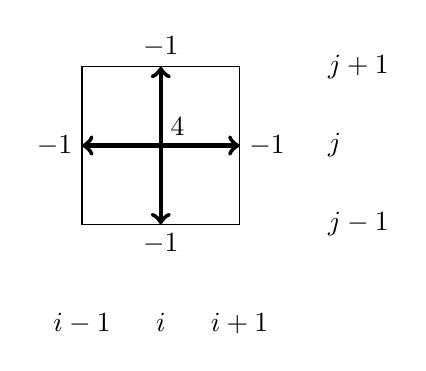
\begin{tikzpicture}
  \draw (0,0) rectangle (2,2);
  \draw [<->, ultra thick] (1,0) -- (1,2);
  \draw [<->, ultra thick] (0,1) -- (2,1);
  
  \node at (1,0) [below] {$-1$};
  \node at (1,2) [above] {$-1$};
  \node at (0,1) [left]  {$-1$};
  \node at (2,1) [right] {$-1$};
  \node at (1,1) [above right] {$4$};
  
  \node at (0,-1) [below] {$i-1$};
  \node at (1,-1) [below] {$i$};
  \node at (2,-1) [below] {$i+1$};

  \node at (3,0) [right] {$j-1$};
  \node at (3,1) [right] {$j$};
  \node at (3,2) [right] {$j+1$};
\end{tikzpicture}
 \\
  \vspace{10mm}
  $
    (Lu)_{i,j} = h^{-2} \left( 4u_{i,j}-u_{i-1,j}-u_{i+1,j}-u_{i,j-1}-u_{i,j+1} \right)
  $
  \end{center}

\end{frame}


\begin{frame}[fragile]
  \frametitle{Jacobi on 2D Poisson}

Assuming homogeneous Dirichlet boundary conditions 
\begin{lstlisting}
for step = 1:nsteps

  for i = 2:n-1
    for j = 2:n-1
      u_next(i,j) = ...
        ( u(i,j+1) + u(i,j-1) + ...
          u(i-1,j) + u(i+1,j) )/4 - ...
        h^2*f(i,j)/4;
    end
  end
  u = u_next;

end
\end{lstlisting}
Basically do some averaging at each step.

\end{frame}


\begin{frame}
  \frametitle{Parallel version (5 point stencil)}
  
  \begin{center}
    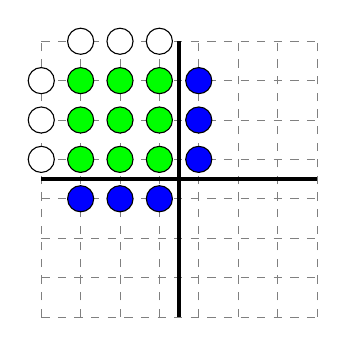
\begin{tikzpicture}
      \draw[step=0.5,gray,very thin,dashed] (0,0) grid (3.5,3.5);
      \draw[ultra thick] (0,1.75) -- (3.5,1.75);
      \draw[ultra thick] (1.75,0) -- (1.75,3.5);
      \begin{scope}[yshift=1.5cm]
      \node[circle,draw=black,fill=white] at (0.5,2.0) {};
\node[circle,draw=black,fill=white] at (1.0,2.0) {};
\node[circle,draw=black,fill=white] at (1.5,2.0) {};

\node[circle,draw=black,fill=white] at (0.0,0.5) {};
\node[circle,draw=black,fill=white] at (0.0,1.0) {};
\node[circle,draw=black,fill=white] at (0.0,1.5) {};

\node[circle,draw=black,fill=green] at (0.5,0.5) {};
\node[circle,draw=black,fill=green] at (0.5,1.0) {};
\node[circle,draw=black,fill=green] at (0.5,1.5) {};
\node[circle,draw=black,fill=green] at (1.0,0.5) {};
\node[circle,draw=black,fill=green] at (1.0,1.0) {};
\node[circle,draw=black,fill=green] at (1.0,1.5) {};
\node[circle,draw=black,fill=green] at (1.5,0.5) {};
\node[circle,draw=black,fill=green] at (1.5,1.0) {};
\node[circle,draw=black,fill=green] at (1.5,1.5) {};

\node[circle,draw=black,fill=blue] at (0.5,0.0) {};
\node[circle,draw=black,fill=blue] at (1.0,0.0) {};
\node[circle,draw=black,fill=blue] at (1.5,0.0) {};

\node[circle,draw=black,fill=blue] at (2.0,0.5) {};
\node[circle,draw=black,fill=blue] at (2.0,1.0) {};
\node[circle,draw=black,fill=blue] at (2.0,1.5) {};

      \end{scope}
    \end{tikzpicture}

  \vspace{5mm}
  \begin{tabular}{ll}
  Boundary values: & white \\
  Data on P0:      & green \\
  Ghost cell data: & blue
  \end{tabular}
  \end{center}

\end{frame}


\begin{frame}
  \frametitle{Parallel version (9 point stencil)}
  
  \begin{center}
    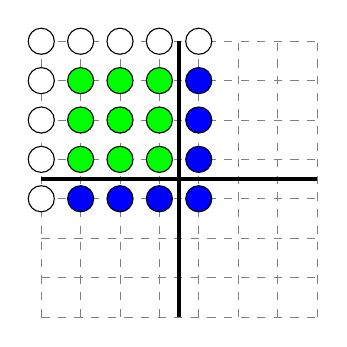
\begin{tikzpicture}
      \draw[step=0.5,gray,very thin,dashed] (0,0) grid (3.5,3.5);
      \draw[ultra thick] (0,1.75) -- (3.5,1.75);
      \draw[ultra thick] (1.75,0) -- (1.75,3.5);
      \begin{scope}
      \node[circle,draw=black,fill=white] at (0.0,3.5) {};      
\node[circle,draw=black,fill=white] at (0.5,3.5) {};
\node[circle,draw=black,fill=white] at (1.0,3.5) {};
\node[circle,draw=black,fill=white] at (1.5,3.5) {};
\node[circle,draw=black,fill=white] at (2.0,3.5) {};

\node[circle,draw=black,fill=white] at (0.0,1.5) {};      
\node[circle,draw=black,fill=white] at (0.0,2.0) {};
\node[circle,draw=black,fill=white] at (0.0,2.5) {};
\node[circle,draw=black,fill=white] at (0.0,3.0) {};

\node[circle,draw=black,fill=green] at (0.5,2.0) {};
\node[circle,draw=black,fill=green] at (0.5,2.5) {};
\node[circle,draw=black,fill=green] at (0.5,3.0) {};
\node[circle,draw=black,fill=green] at (1.0,2.0) {};
\node[circle,draw=black,fill=green] at (1.0,2.5) {};
\node[circle,draw=black,fill=green] at (1.0,3.0) {};
\node[circle,draw=black,fill=green] at (1.5,2.0) {};
\node[circle,draw=black,fill=green] at (1.5,2.5) {};
\node[circle,draw=black,fill=green] at (1.5,3.0) {};

\node[circle,draw=black,fill=blue] at (0.5,1.5) {};
\node[circle,draw=black,fill=blue] at (1.0,1.5) {};
\node[circle,draw=black,fill=blue] at (1.5,1.5) {};

\node[circle,draw=black,fill=blue] at (2.0,1.5) {};      
\node[circle,draw=black,fill=blue] at (2.0,2.0) {};
\node[circle,draw=black,fill=blue] at (2.0,2.5) {};
\node[circle,draw=black,fill=blue] at (2.0,3.0) {};      

      \end{scope}
    \end{tikzpicture}

  \vspace{5mm}
  \begin{tabular}{ll}
  Boundary values: & white \\
  Data on P0:      & green \\
  Ghost cell data: & blue
  \end{tabular}
  \end{center}

\end{frame}


\begin{frame}
  \frametitle{Parallel version (5 point stencil)}

  \begin{center}
    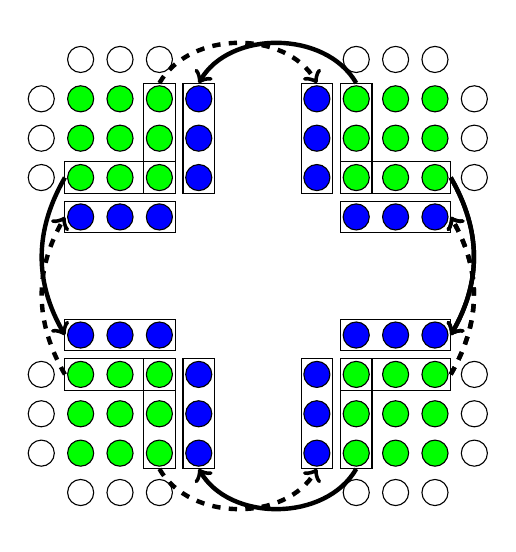
\begin{tikzpicture}

  \begin{scope}[yshift=3.5cm]
    \node[circle,draw=black,fill=white] at (0.5,2.0) {};
\node[circle,draw=black,fill=white] at (1.0,2.0) {};
\node[circle,draw=black,fill=white] at (1.5,2.0) {};

\node[circle,draw=black,fill=white] at (0.0,0.5) {};
\node[circle,draw=black,fill=white] at (0.0,1.0) {};
\node[circle,draw=black,fill=white] at (0.0,1.5) {};

\node[circle,draw=black,fill=green] at (0.5,0.5) {};
\node[circle,draw=black,fill=green] at (0.5,1.0) {};
\node[circle,draw=black,fill=green] at (0.5,1.5) {};
\node[circle,draw=black,fill=green] at (1.0,0.5) {};
\node[circle,draw=black,fill=green] at (1.0,1.0) {};
\node[circle,draw=black,fill=green] at (1.0,1.5) {};
\node[circle,draw=black,fill=green] at (1.5,0.5) {};
\node[circle,draw=black,fill=green] at (1.5,1.0) {};
\node[circle,draw=black,fill=green] at (1.5,1.5) {};

\node[circle,draw=black,fill=blue] at (0.5,0.0) {};
\node[circle,draw=black,fill=blue] at (1.0,0.0) {};
\node[circle,draw=black,fill=blue] at (1.5,0.0) {};

\node[circle,draw=black,fill=blue] at (2.0,0.5) {};
\node[circle,draw=black,fill=blue] at (2.0,1.0) {};
\node[circle,draw=black,fill=blue] at (2.0,1.5) {};

  \end{scope}
  
  \begin{scope}[xshift=2.0cm]
  \begin{scope}[rotate=90]
    \node[circle,draw=black,fill=white] at (0.5,2.0) {};
\node[circle,draw=black,fill=white] at (1.0,2.0) {};
\node[circle,draw=black,fill=white] at (1.5,2.0) {};

\node[circle,draw=black,fill=white] at (0.0,0.5) {};
\node[circle,draw=black,fill=white] at (0.0,1.0) {};
\node[circle,draw=black,fill=white] at (0.0,1.5) {};

\node[circle,draw=black,fill=green] at (0.5,0.5) {};
\node[circle,draw=black,fill=green] at (0.5,1.0) {};
\node[circle,draw=black,fill=green] at (0.5,1.5) {};
\node[circle,draw=black,fill=green] at (1.0,0.5) {};
\node[circle,draw=black,fill=green] at (1.0,1.0) {};
\node[circle,draw=black,fill=green] at (1.0,1.5) {};
\node[circle,draw=black,fill=green] at (1.5,0.5) {};
\node[circle,draw=black,fill=green] at (1.5,1.0) {};
\node[circle,draw=black,fill=green] at (1.5,1.5) {};

\node[circle,draw=black,fill=blue] at (0.5,0.0) {};
\node[circle,draw=black,fill=blue] at (1.0,0.0) {};
\node[circle,draw=black,fill=blue] at (1.5,0.0) {};

\node[circle,draw=black,fill=blue] at (2.0,0.5) {};
\node[circle,draw=black,fill=blue] at (2.0,1.0) {};
\node[circle,draw=black,fill=blue] at (2.0,1.5) {};

  \end{scope}
  \end{scope}

  \begin{scope}[xshift=3.5cm,yshift=5.5cm]
  \begin{scope}[rotate=-90]
    \node[circle,draw=black,fill=white] at (0.5,2.0) {};
\node[circle,draw=black,fill=white] at (1.0,2.0) {};
\node[circle,draw=black,fill=white] at (1.5,2.0) {};

\node[circle,draw=black,fill=white] at (0.0,0.5) {};
\node[circle,draw=black,fill=white] at (0.0,1.0) {};
\node[circle,draw=black,fill=white] at (0.0,1.5) {};

\node[circle,draw=black,fill=green] at (0.5,0.5) {};
\node[circle,draw=black,fill=green] at (0.5,1.0) {};
\node[circle,draw=black,fill=green] at (0.5,1.5) {};
\node[circle,draw=black,fill=green] at (1.0,0.5) {};
\node[circle,draw=black,fill=green] at (1.0,1.0) {};
\node[circle,draw=black,fill=green] at (1.0,1.5) {};
\node[circle,draw=black,fill=green] at (1.5,0.5) {};
\node[circle,draw=black,fill=green] at (1.5,1.0) {};
\node[circle,draw=black,fill=green] at (1.5,1.5) {};

\node[circle,draw=black,fill=blue] at (0.5,0.0) {};
\node[circle,draw=black,fill=blue] at (1.0,0.0) {};
\node[circle,draw=black,fill=blue] at (1.5,0.0) {};

\node[circle,draw=black,fill=blue] at (2.0,0.5) {};
\node[circle,draw=black,fill=blue] at (2.0,1.0) {};
\node[circle,draw=black,fill=blue] at (2.0,1.5) {};

  \end{scope}
  \end{scope}

  \begin{scope}[xshift=5.5cm,yshift=2.0cm]
  \begin{scope}[rotate=180]
    \node[circle,draw=black,fill=white] at (0.5,2.0) {};
\node[circle,draw=black,fill=white] at (1.0,2.0) {};
\node[circle,draw=black,fill=white] at (1.5,2.0) {};

\node[circle,draw=black,fill=white] at (0.0,0.5) {};
\node[circle,draw=black,fill=white] at (0.0,1.0) {};
\node[circle,draw=black,fill=white] at (0.0,1.5) {};

\node[circle,draw=black,fill=green] at (0.5,0.5) {};
\node[circle,draw=black,fill=green] at (0.5,1.0) {};
\node[circle,draw=black,fill=green] at (0.5,1.5) {};
\node[circle,draw=black,fill=green] at (1.0,0.5) {};
\node[circle,draw=black,fill=green] at (1.0,1.0) {};
\node[circle,draw=black,fill=green] at (1.0,1.5) {};
\node[circle,draw=black,fill=green] at (1.5,0.5) {};
\node[circle,draw=black,fill=green] at (1.5,1.0) {};
\node[circle,draw=black,fill=green] at (1.5,1.5) {};

\node[circle,draw=black,fill=blue] at (0.5,0.0) {};
\node[circle,draw=black,fill=blue] at (1.0,0.0) {};
\node[circle,draw=black,fill=blue] at (1.5,0.0) {};

\node[circle,draw=black,fill=blue] at (2.0,0.5) {};
\node[circle,draw=black,fill=blue] at (2.0,1.0) {};
\node[circle,draw=black,fill=blue] at (2.0,1.5) {};

  \end{scope}      
  \end{scope}

  \draw (0.3,1.8) rectangle (1.7,2.2);  % SW ghost (top)
  \draw (0.3,1.3) rectangle (1.7,1.7);  % SW data  (top)

  \draw (1.8,0.3) rectangle (2.2,1.7);  % SW ghost (right)
  \draw (1.3,0.3) rectangle (1.7,1.7);  % SW data  (right)
  
  \draw (0.3,3.8) rectangle (1.7,4.2);  % NW data  (bottom)
  \draw (0.3,3.3) rectangle (1.7,3.7);  % NW ghost (bottom)

  \draw (1.8,3.8) rectangle (2.2,5.2);  % NW ghost (right)
  \draw (1.3,3.8) rectangle (1.7,5.2);  % NW data  (right)

  \draw (3.8,1.8) rectangle (5.2,2.2);  % SE ghost (top)
  \draw (3.8,1.3) rectangle (5.2,1.7);  % SE data  (top)

  \draw (3.8,0.3) rectangle (4.2,1.7);  % SE data  (left)
  \draw (3.3,0.3) rectangle (3.7,1.7);  % SE ghost (left)
  
  \draw (3.8,3.8) rectangle (5.2,4.2);  % NE data  (bottom)
  \draw (3.8,3.3) rectangle (5.2,3.7);  % NE ghost (bottom)

  \draw (3.8,3.8) rectangle (4.2,5.2);  % NE data  (left)
  \draw (3.3,3.8) rectangle (3.7,5.2);  % NE ghost (left)

  % SW/NW exchange
  \draw[ultra thick,->] (0.3,4.0) to [out=-120,in=120] (0.3,2.0);
  \draw[ultra thick,dashed,->] (0.3,1.5) to [out=120,in=-120] (0.3,3.5);

  % SE/NE exchange
  \draw[ultra thick,->] (5.2,4.0) to [out=-60,in=60] (5.2,2.0);
  \draw[ultra thick,dashed,->] (5.2,1.5) to [out=60,in=-60] (5.2,3.5);

  % SE/SW exchange
  \draw[ultra thick,->] (4.0,0.3) to [out=-120,in=-60] (2.0,0.3);
  \draw[ultra thick,dashed,->] (1.5,0.3) to [out=-60,in=-120] (3.5,0.3);

  % SE/NE exchange
  \draw[ultra thick,->] (5.2,4.0) to [out=-60,in=60] (5.2,2.0);
  \draw[ultra thick,dashed,->] (5.2,1.5) to [out=60,in=-60] (5.2,3.5);

  % NE/NW exchange
  \draw[ultra thick,->] (4.0,5.2) to [out=120,in=60] (2.0,5.2);
  \draw[ultra thick,dashed,->] (1.5,5.2) to [out=60,in=120] (3.5,5.2);
  
\end{tikzpicture}


    Communicate ghost cells before each step.
  \end{center}
\end{frame}


\begin{frame}
  \frametitle{Parallel version (9 point stencil)}

  \begin{center}
    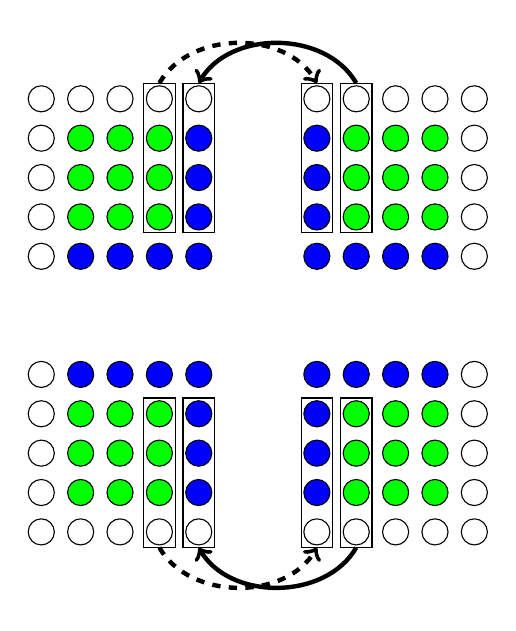
\begin{tikzpicture}

  \begin{scope}[yshift=2.0cm]
    \node[circle,draw=black,fill=white] at (0.0,3.5) {};      
\node[circle,draw=black,fill=white] at (0.5,3.5) {};
\node[circle,draw=black,fill=white] at (1.0,3.5) {};
\node[circle,draw=black,fill=white] at (1.5,3.5) {};
\node[circle,draw=black,fill=white] at (2.0,3.5) {};

\node[circle,draw=black,fill=white] at (0.0,1.5) {};      
\node[circle,draw=black,fill=white] at (0.0,2.0) {};
\node[circle,draw=black,fill=white] at (0.0,2.5) {};
\node[circle,draw=black,fill=white] at (0.0,3.0) {};

\node[circle,draw=black,fill=green] at (0.5,2.0) {};
\node[circle,draw=black,fill=green] at (0.5,2.5) {};
\node[circle,draw=black,fill=green] at (0.5,3.0) {};
\node[circle,draw=black,fill=green] at (1.0,2.0) {};
\node[circle,draw=black,fill=green] at (1.0,2.5) {};
\node[circle,draw=black,fill=green] at (1.0,3.0) {};
\node[circle,draw=black,fill=green] at (1.5,2.0) {};
\node[circle,draw=black,fill=green] at (1.5,2.5) {};
\node[circle,draw=black,fill=green] at (1.5,3.0) {};

\node[circle,draw=black,fill=blue] at (0.5,1.5) {};
\node[circle,draw=black,fill=blue] at (1.0,1.5) {};
\node[circle,draw=black,fill=blue] at (1.5,1.5) {};

\node[circle,draw=black,fill=blue] at (2.0,1.5) {};      
\node[circle,draw=black,fill=blue] at (2.0,2.0) {};
\node[circle,draw=black,fill=blue] at (2.0,2.5) {};
\node[circle,draw=black,fill=blue] at (2.0,3.0) {};      

  \end{scope}
  
  \begin{scope}[xshift=3.5cm]
  \begin{scope}[rotate=90]
    \node[circle,draw=black,fill=white] at (0.0,3.5) {};      
\node[circle,draw=black,fill=white] at (0.5,3.5) {};
\node[circle,draw=black,fill=white] at (1.0,3.5) {};
\node[circle,draw=black,fill=white] at (1.5,3.5) {};
\node[circle,draw=black,fill=white] at (2.0,3.5) {};

\node[circle,draw=black,fill=white] at (0.0,1.5) {};      
\node[circle,draw=black,fill=white] at (0.0,2.0) {};
\node[circle,draw=black,fill=white] at (0.0,2.5) {};
\node[circle,draw=black,fill=white] at (0.0,3.0) {};

\node[circle,draw=black,fill=green] at (0.5,2.0) {};
\node[circle,draw=black,fill=green] at (0.5,2.5) {};
\node[circle,draw=black,fill=green] at (0.5,3.0) {};
\node[circle,draw=black,fill=green] at (1.0,2.0) {};
\node[circle,draw=black,fill=green] at (1.0,2.5) {};
\node[circle,draw=black,fill=green] at (1.0,3.0) {};
\node[circle,draw=black,fill=green] at (1.5,2.0) {};
\node[circle,draw=black,fill=green] at (1.5,2.5) {};
\node[circle,draw=black,fill=green] at (1.5,3.0) {};

\node[circle,draw=black,fill=blue] at (0.5,1.5) {};
\node[circle,draw=black,fill=blue] at (1.0,1.5) {};
\node[circle,draw=black,fill=blue] at (1.5,1.5) {};

\node[circle,draw=black,fill=blue] at (2.0,1.5) {};      
\node[circle,draw=black,fill=blue] at (2.0,2.0) {};
\node[circle,draw=black,fill=blue] at (2.0,2.5) {};
\node[circle,draw=black,fill=blue] at (2.0,3.0) {};      

  \end{scope}
  \end{scope}

  \begin{scope}[xshift=2.0cm,yshift=5.5cm]
  \begin{scope}[rotate=-90]
    \node[circle,draw=black,fill=white] at (0.0,3.5) {};      
\node[circle,draw=black,fill=white] at (0.5,3.5) {};
\node[circle,draw=black,fill=white] at (1.0,3.5) {};
\node[circle,draw=black,fill=white] at (1.5,3.5) {};
\node[circle,draw=black,fill=white] at (2.0,3.5) {};

\node[circle,draw=black,fill=white] at (0.0,1.5) {};      
\node[circle,draw=black,fill=white] at (0.0,2.0) {};
\node[circle,draw=black,fill=white] at (0.0,2.5) {};
\node[circle,draw=black,fill=white] at (0.0,3.0) {};

\node[circle,draw=black,fill=green] at (0.5,2.0) {};
\node[circle,draw=black,fill=green] at (0.5,2.5) {};
\node[circle,draw=black,fill=green] at (0.5,3.0) {};
\node[circle,draw=black,fill=green] at (1.0,2.0) {};
\node[circle,draw=black,fill=green] at (1.0,2.5) {};
\node[circle,draw=black,fill=green] at (1.0,3.0) {};
\node[circle,draw=black,fill=green] at (1.5,2.0) {};
\node[circle,draw=black,fill=green] at (1.5,2.5) {};
\node[circle,draw=black,fill=green] at (1.5,3.0) {};

\node[circle,draw=black,fill=blue] at (0.5,1.5) {};
\node[circle,draw=black,fill=blue] at (1.0,1.5) {};
\node[circle,draw=black,fill=blue] at (1.5,1.5) {};

\node[circle,draw=black,fill=blue] at (2.0,1.5) {};      
\node[circle,draw=black,fill=blue] at (2.0,2.0) {};
\node[circle,draw=black,fill=blue] at (2.0,2.5) {};
\node[circle,draw=black,fill=blue] at (2.0,3.0) {};      

  \end{scope}
  \end{scope}

  \begin{scope}[xshift=5.5cm,yshift=3.5cm]
  \begin{scope}[rotate=180]
    \node[circle,draw=black,fill=white] at (0.0,3.5) {};      
\node[circle,draw=black,fill=white] at (0.5,3.5) {};
\node[circle,draw=black,fill=white] at (1.0,3.5) {};
\node[circle,draw=black,fill=white] at (1.5,3.5) {};
\node[circle,draw=black,fill=white] at (2.0,3.5) {};

\node[circle,draw=black,fill=white] at (0.0,1.5) {};      
\node[circle,draw=black,fill=white] at (0.0,2.0) {};
\node[circle,draw=black,fill=white] at (0.0,2.5) {};
\node[circle,draw=black,fill=white] at (0.0,3.0) {};

\node[circle,draw=black,fill=green] at (0.5,2.0) {};
\node[circle,draw=black,fill=green] at (0.5,2.5) {};
\node[circle,draw=black,fill=green] at (0.5,3.0) {};
\node[circle,draw=black,fill=green] at (1.0,2.0) {};
\node[circle,draw=black,fill=green] at (1.0,2.5) {};
\node[circle,draw=black,fill=green] at (1.0,3.0) {};
\node[circle,draw=black,fill=green] at (1.5,2.0) {};
\node[circle,draw=black,fill=green] at (1.5,2.5) {};
\node[circle,draw=black,fill=green] at (1.5,3.0) {};

\node[circle,draw=black,fill=blue] at (0.5,1.5) {};
\node[circle,draw=black,fill=blue] at (1.0,1.5) {};
\node[circle,draw=black,fill=blue] at (1.5,1.5) {};

\node[circle,draw=black,fill=blue] at (2.0,1.5) {};      
\node[circle,draw=black,fill=blue] at (2.0,2.0) {};
\node[circle,draw=black,fill=blue] at (2.0,2.5) {};
\node[circle,draw=black,fill=blue] at (2.0,3.0) {};      

  \end{scope}      
  \end{scope}

  \draw (1.8,-0.2) rectangle (2.2,1.7);  % SW ghost (right)
  \draw (1.3,-0.2) rectangle (1.7,1.7);  % SW data  (right)
  
  \draw (1.8,3.8) rectangle (2.2,5.7);  % NW ghost (right)
  \draw (1.3,3.8) rectangle (1.7,5.7);  % NW data  (right)

  \draw (3.8,-0.2) rectangle (4.2,1.7);  % SE data  (left)
  \draw (3.3,-0.2) rectangle (3.7,1.7);  % SE ghost (left)
  
  \draw (3.8,3.8) rectangle (4.2,5.7);  % NE data  (left)
  \draw (3.3,3.8) rectangle (3.7,5.7);  % NE ghost (left)

  % SE/SW exchange
  \draw[ultra thick,->] (4.0,-0.2) to [out=-120,in=-60] (2.0,-0.2);
  \draw[ultra thick,dashed,->] (1.5,-0.2) to [out=-60,in=-120] (3.5,-0.2);

  % NE/NW exchange
  \draw[ultra thick,->] (4.0,5.7) to [out=120,in=60] (2.0,5.7);
  \draw[ultra thick,dashed,->] (1.5,5.7) to [out=60,in=120] (3.5,5.7);
  
\end{tikzpicture}

    
  Communicate in two phases (\alert{EW}, NS) to get corners.
  \end{center}
\end{frame}


\begin{frame}
  \frametitle{Parallel version (9 point stencil)}

  \begin{center}
    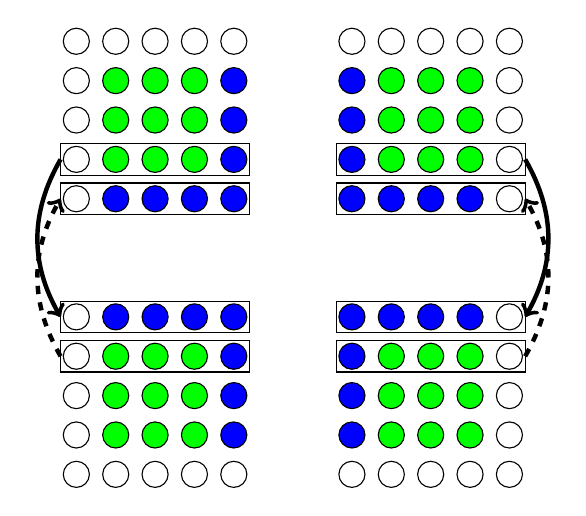
\begin{tikzpicture}
  \begin{scope}[yshift=2.0cm]
    \node[circle,draw=black,fill=white] at (0.0,3.5) {};      
\node[circle,draw=black,fill=white] at (0.5,3.5) {};
\node[circle,draw=black,fill=white] at (1.0,3.5) {};
\node[circle,draw=black,fill=white] at (1.5,3.5) {};
\node[circle,draw=black,fill=white] at (2.0,3.5) {};

\node[circle,draw=black,fill=white] at (0.0,1.5) {};      
\node[circle,draw=black,fill=white] at (0.0,2.0) {};
\node[circle,draw=black,fill=white] at (0.0,2.5) {};
\node[circle,draw=black,fill=white] at (0.0,3.0) {};

\node[circle,draw=black,fill=green] at (0.5,2.0) {};
\node[circle,draw=black,fill=green] at (0.5,2.5) {};
\node[circle,draw=black,fill=green] at (0.5,3.0) {};
\node[circle,draw=black,fill=green] at (1.0,2.0) {};
\node[circle,draw=black,fill=green] at (1.0,2.5) {};
\node[circle,draw=black,fill=green] at (1.0,3.0) {};
\node[circle,draw=black,fill=green] at (1.5,2.0) {};
\node[circle,draw=black,fill=green] at (1.5,2.5) {};
\node[circle,draw=black,fill=green] at (1.5,3.0) {};

\node[circle,draw=black,fill=blue] at (0.5,1.5) {};
\node[circle,draw=black,fill=blue] at (1.0,1.5) {};
\node[circle,draw=black,fill=blue] at (1.5,1.5) {};

\node[circle,draw=black,fill=blue] at (2.0,1.5) {};      
\node[circle,draw=black,fill=blue] at (2.0,2.0) {};
\node[circle,draw=black,fill=blue] at (2.0,2.5) {};
\node[circle,draw=black,fill=blue] at (2.0,3.0) {};      

  \end{scope}
  
  \begin{scope}[xshift=3.5cm]
  \begin{scope}[rotate=90]
    \node[circle,draw=black,fill=white] at (0.0,3.5) {};      
\node[circle,draw=black,fill=white] at (0.5,3.5) {};
\node[circle,draw=black,fill=white] at (1.0,3.5) {};
\node[circle,draw=black,fill=white] at (1.5,3.5) {};
\node[circle,draw=black,fill=white] at (2.0,3.5) {};

\node[circle,draw=black,fill=white] at (0.0,1.5) {};      
\node[circle,draw=black,fill=white] at (0.0,2.0) {};
\node[circle,draw=black,fill=white] at (0.0,2.5) {};
\node[circle,draw=black,fill=white] at (0.0,3.0) {};

\node[circle,draw=black,fill=green] at (0.5,2.0) {};
\node[circle,draw=black,fill=green] at (0.5,2.5) {};
\node[circle,draw=black,fill=green] at (0.5,3.0) {};
\node[circle,draw=black,fill=green] at (1.0,2.0) {};
\node[circle,draw=black,fill=green] at (1.0,2.5) {};
\node[circle,draw=black,fill=green] at (1.0,3.0) {};
\node[circle,draw=black,fill=green] at (1.5,2.0) {};
\node[circle,draw=black,fill=green] at (1.5,2.5) {};
\node[circle,draw=black,fill=green] at (1.5,3.0) {};

\node[circle,draw=black,fill=blue] at (0.5,1.5) {};
\node[circle,draw=black,fill=blue] at (1.0,1.5) {};
\node[circle,draw=black,fill=blue] at (1.5,1.5) {};

\node[circle,draw=black,fill=blue] at (2.0,1.5) {};      
\node[circle,draw=black,fill=blue] at (2.0,2.0) {};
\node[circle,draw=black,fill=blue] at (2.0,2.5) {};
\node[circle,draw=black,fill=blue] at (2.0,3.0) {};      

  \end{scope}
  \end{scope}

  \begin{scope}[xshift=2.0cm,yshift=5.5cm]
  \begin{scope}[rotate=-90]
    \node[circle,draw=black,fill=white] at (0.0,3.5) {};      
\node[circle,draw=black,fill=white] at (0.5,3.5) {};
\node[circle,draw=black,fill=white] at (1.0,3.5) {};
\node[circle,draw=black,fill=white] at (1.5,3.5) {};
\node[circle,draw=black,fill=white] at (2.0,3.5) {};

\node[circle,draw=black,fill=white] at (0.0,1.5) {};      
\node[circle,draw=black,fill=white] at (0.0,2.0) {};
\node[circle,draw=black,fill=white] at (0.0,2.5) {};
\node[circle,draw=black,fill=white] at (0.0,3.0) {};

\node[circle,draw=black,fill=green] at (0.5,2.0) {};
\node[circle,draw=black,fill=green] at (0.5,2.5) {};
\node[circle,draw=black,fill=green] at (0.5,3.0) {};
\node[circle,draw=black,fill=green] at (1.0,2.0) {};
\node[circle,draw=black,fill=green] at (1.0,2.5) {};
\node[circle,draw=black,fill=green] at (1.0,3.0) {};
\node[circle,draw=black,fill=green] at (1.5,2.0) {};
\node[circle,draw=black,fill=green] at (1.5,2.5) {};
\node[circle,draw=black,fill=green] at (1.5,3.0) {};

\node[circle,draw=black,fill=blue] at (0.5,1.5) {};
\node[circle,draw=black,fill=blue] at (1.0,1.5) {};
\node[circle,draw=black,fill=blue] at (1.5,1.5) {};

\node[circle,draw=black,fill=blue] at (2.0,1.5) {};      
\node[circle,draw=black,fill=blue] at (2.0,2.0) {};
\node[circle,draw=black,fill=blue] at (2.0,2.5) {};
\node[circle,draw=black,fill=blue] at (2.0,3.0) {};      

  \end{scope}
  \end{scope}

  \begin{scope}[xshift=5.5cm,yshift=3.5cm]
  \begin{scope}[rotate=180]
    \node[circle,draw=black,fill=white] at (0.0,3.5) {};      
\node[circle,draw=black,fill=white] at (0.5,3.5) {};
\node[circle,draw=black,fill=white] at (1.0,3.5) {};
\node[circle,draw=black,fill=white] at (1.5,3.5) {};
\node[circle,draw=black,fill=white] at (2.0,3.5) {};

\node[circle,draw=black,fill=white] at (0.0,1.5) {};      
\node[circle,draw=black,fill=white] at (0.0,2.0) {};
\node[circle,draw=black,fill=white] at (0.0,2.5) {};
\node[circle,draw=black,fill=white] at (0.0,3.0) {};

\node[circle,draw=black,fill=green] at (0.5,2.0) {};
\node[circle,draw=black,fill=green] at (0.5,2.5) {};
\node[circle,draw=black,fill=green] at (0.5,3.0) {};
\node[circle,draw=black,fill=green] at (1.0,2.0) {};
\node[circle,draw=black,fill=green] at (1.0,2.5) {};
\node[circle,draw=black,fill=green] at (1.0,3.0) {};
\node[circle,draw=black,fill=green] at (1.5,2.0) {};
\node[circle,draw=black,fill=green] at (1.5,2.5) {};
\node[circle,draw=black,fill=green] at (1.5,3.0) {};

\node[circle,draw=black,fill=blue] at (0.5,1.5) {};
\node[circle,draw=black,fill=blue] at (1.0,1.5) {};
\node[circle,draw=black,fill=blue] at (1.5,1.5) {};

\node[circle,draw=black,fill=blue] at (2.0,1.5) {};      
\node[circle,draw=black,fill=blue] at (2.0,2.0) {};
\node[circle,draw=black,fill=blue] at (2.0,2.5) {};
\node[circle,draw=black,fill=blue] at (2.0,3.0) {};      

  \end{scope}      
  \end{scope}

  \draw (-0.2,1.8) rectangle (2.2,2.2);  % SW ghost (top)
  \draw (-0.2,1.3) rectangle (2.2,1.7);  % SW data  (top)
  
  \draw (-0.2,3.8) rectangle (2.2,4.2);  % NW data  (bottom)
  \draw (-0.2,3.3) rectangle (2.2,3.7);  % NW ghost (bottom)

  \draw (3.3,1.8) rectangle (5.7,2.2);  % SE ghost (top)
  \draw (3.3,1.3) rectangle (5.7,1.7);  % SE data  (top)

  \draw (3.3,3.8) rectangle (5.7,4.2);  % NE data  (bottom)
  \draw (3.3,3.3) rectangle (5.7,3.7);  % NE ghost (bottom)

  % SW/NW exchange
  \draw[ultra thick,->] (-0.2,4.0) to [out=-120,in=120] (-0.2,2.0);
  \draw[ultra thick,dashed,->] (-0.2,1.5) to [out=120,in=-120] (-0.2,3.5);

  % SE/NE exchange
  \draw[ultra thick,->] (5.7,4.0) to [out=-60,in=60] (5.7,2.0);
  \draw[ultra thick,dashed,->] (5.7,1.5) to [out=60,in=-60] (5.7,3.5);

\end{tikzpicture}


  Communicate in two phases (EW, \alert{NS}) to get corners.
  \end{center}
\end{frame}


\begin{frame}[fragile]
  \frametitle{Gauss-Seidel on 2D Poisson}

\begin{lstlisting}
for step = 1:nsteps

  for i = 2:n-1
    for j = 2:n-1
      u(i,j) = ...
        ( u(i,j+1) + u(i,j-1) + ...
          u(i-1,j) + u(i+1,j) )/4 - ...
        h^2*f(i,j)/4;
    end
  end

end
\end{lstlisting}
Bottom values depend on top; how to parallelize?

\end{frame}


\begin{frame}[fragile]
  \frametitle{Red-Black Gauss-Seidel}

  \begin{center}
    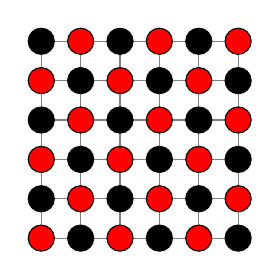
\begin{tikzpicture}
  \draw[step=0.5,gray] (0,0) grid (2.5,2.5);

  \node[circle,draw=black,fill=red]   at (0.0,0.0) {};      
  \node[circle,draw=black,fill=black] at (0.5,0.0) {};      
  \node[circle,draw=black,fill=red]   at (1.0,0.0) {};      
  \node[circle,draw=black,fill=black] at (1.5,0.0) {};      
  \node[circle,draw=black,fill=red]   at (2.0,0.0) {};      
  \node[circle,draw=black,fill=black] at (2.5,0.0) {};      
  \node[circle,draw=black,fill=black] at (0.0,0.5) {};      
  \node[circle,draw=black,fill=red]   at (0.5,0.5) {};      
  \node[circle,draw=black,fill=black] at (1.0,0.5) {};      
  \node[circle,draw=black,fill=red]   at (1.5,0.5) {};      
  \node[circle,draw=black,fill=black] at (2.0,0.5) {};      
  \node[circle,draw=black,fill=red]   at (2.5,0.5) {};      
  \node[circle,draw=black,fill=red]   at (0.0,1.0) {};      
  \node[circle,draw=black,fill=black] at (0.5,1.0) {};      
  \node[circle,draw=black,fill=red]   at (1.0,1.0) {};      
  \node[circle,draw=black,fill=black] at (1.5,1.0) {};      
  \node[circle,draw=black,fill=red]   at (2.0,1.0) {};      
  \node[circle,draw=black,fill=black] at (2.5,1.0) {};      
  \node[circle,draw=black,fill=black] at (0.0,1.5) {};      
  \node[circle,draw=black,fill=red]   at (0.5,1.5) {};      
  \node[circle,draw=black,fill=black] at (1.0,1.5) {};      
  \node[circle,draw=black,fill=red]   at (1.5,1.5) {};      
  \node[circle,draw=black,fill=black] at (2.0,1.5) {};      
  \node[circle,draw=black,fill=red]   at (2.5,1.5) {};      
  \node[circle,draw=black,fill=red]   at (0.0,2.0) {};      
  \node[circle,draw=black,fill=black] at (0.5,2.0) {};      
  \node[circle,draw=black,fill=red]   at (1.0,2.0) {};      
  \node[circle,draw=black,fill=black] at (1.5,2.0) {};      
  \node[circle,draw=black,fill=red]   at (2.0,2.0) {};      
  \node[circle,draw=black,fill=black] at (2.5,2.0) {};      
  \node[circle,draw=black,fill=black] at (0.0,2.5) {};      
  \node[circle,draw=black,fill=red]   at (0.5,2.5) {};      
  \node[circle,draw=black,fill=black] at (1.0,2.5) {};      
  \node[circle,draw=black,fill=red]   at (1.5,2.5) {};      
  \node[circle,draw=black,fill=black] at (2.0,2.5) {};      
  \node[circle,draw=black,fill=red]   at (2.5,2.5) {};      

\end{tikzpicture}


  \vspace{5mm}
  Red depends only on black, and vice-versa. \\
  Generalization: multi-color orderings
  \end{center}
\end{frame}


\begin{frame}[fragile]
  \frametitle{Red black Gauss-Seidel step}

\begin{lstlisting}
  for i = 2:n-1
    for j = 2:n-1
      if mod(i+j,2) == 0
        u(i,j) = ...
      end
    end
  end

  for i = 2:n-1
    for j = 2:n-1
      if mod(i+j,2) == 1,
      u(i,j) = ...
    end
  end
\end{lstlisting}

\end{frame}

\begin{frame}
  \frametitle{Parallel red-black Gauss-Seidel sketch}

  At each step
  \begin{itemize}
  \item Send black ghost cells
  \item Update red cells
  \item Send red ghost cells
  \item Update black ghost cells
  \end{itemize}
\end{frame}


\begin{frame}
  \frametitle{More Sophistication}

  \begin{itemize}
  \item Successive over-relaxation (SOR): extrapolate Gauss-Seidel direction
  \item Block Jacobi: let $M$ be a block diagonal matrix from $A$
    \begin{itemize}
    \item Other block variants similar
    \end{itemize}
  \item Alternating Direction Implicit (ADI): alternately solve on vertical
    lines and horizontal lines
  \item Multigrid
  \end{itemize}
  These are mostly just the opening act for...
\end{frame}


\begin{frame}
  \frametitle{Krylov Subspace Methods}

  What if we only know how to multiply by $A$? \\
  About all you can do is keep multiplying!
  \[
    \mathcal{K}_k(A,b) = \operatorname{span}\left\{ 
      b, A b, A^2 b, \ldots, A^{k-1} b \right\}.
  \]
  Gives surprisingly useful information!

\end{frame}


\begin{frame}
  \frametitle{Example: Conjugate Gradients}

  If $A$ is symmetric and positive definite,
  $Ax = b$ solves a minimization:
  \begin{align*}
    \phi(x) &= \frac{1}{2} x^T A x - x^T  b\\
    \nabla \phi(x) &= Ax - b.
  \end{align*}
  Idea: Minimize $\phi(x)$ over $\mathcal{K}_k(A,b)$. \\
  Basis for the {\em method of conjugate gradients}
\end{frame}


\begin{frame}
  \frametitle{Example: GMRES}

  Idea: Minimize $\|Ax-b\|^2$ over $\mathcal{K}_k(A,b)$. \\
  Yields {\em Generalized Minimum RESidual} (GMRES) method.
\end{frame}


\begin{frame}
  \frametitle{Convergence of Krylov Subspace Methods}

  \begin{itemize}
  \item KSPs are {\em not} stationary (no constant fixed-point iteration)
  \item Convergence is surprisingly subtle!
  \item CG convergence upper bound via {\em condition number}
    \begin{itemize}
    \item Large condition number iff form $\phi(x)$ has long narrow bowl
    \item Usually happens for Poisson and related problems
    \end{itemize}
  \item {\em Preconditioned} problem
    $M^{-1} A x = M^{-1} b$ converges faster?
  \item Whence $M$?  
    \begin{itemize}
    \item From a stationary method?
    \item From a simpler/coarser discretization?
    \item From approximate factorization?
    \end{itemize}
  \end{itemize}
\end{frame}


\begin{frame}[fragile]
  \frametitle{PCG}

\begin{minipage}{0.6\textwidth}
\begin{tabbing}
Compute $r^{(0)} = b - Ax$ \\
for \= $i = 1, 2, \ldots$ \\
\> solve $Mz^{(i-1)} = r^{(i-1)}$ \\
\> $\rho_{i-1} = (r^{(i-1)})^T z^{(i-1)}$ \\
\> if \= $i == 1$ \\
\> \> $p^{(1)} = z^{(0)}$ \\
\> else \\
\> \> $\beta_{i-1} = \rho_{i-1}/\rho_{i-2}$ \\
\> \> $p^{(i)} = z^{(i-1)} + \beta_{i-1} p^{(i-1)}$ \\
\> endif \\
\> $q^{(i)} = A p^{(i)}$ \\
\> $\alpha_i = \rho_{i-1} / (p^{(i)})^T q^{(i)}$ \\
\> $x^{(i)} = x^{(i-1)} + \alpha_i p^{(i)}$ \\
\> $r^{(i)} = r^{(i-1)} - \alpha_i q^{(i)}$ \\
end
\end{tabbing}
\end{minipage}
\begin{minipage}{0.35\textwidth}
  Parallel work:
  \begin{itemize}
    \item Solve with $M$
    \item Product with $A$
    \item Dot products
    \item Axpys
  \end{itemize}
  Overlap comm/comp.
\end{minipage}

\end{frame}


\begin{frame}[fragile]
  \frametitle{PCG bottlenecks}

  Key: fast solve with $M$, product with $A$
  \begin{itemize}
  \item Some preconditioners parallelize better! \\
    (Jacobi vs Gauss-Seidel)
  \item Balance speed with performance.
    \begin{itemize}
    \item Speed for set up of $M$?
    \item Speed to apply $M$ after setup?
    \end{itemize}
  \item Cheaper to do two multiplies/solves at once...
    \begin{itemize}
    \item Can't exploit in obvious way --- lose stability
    \item Variants allow multiple products --- Hoemmen's thesis
    \end{itemize}
  \item Lots of fiddling possible with $M$; 
    matvec with $A$?
  \end{itemize}

\end{frame}

\end{document}
